% LDraw-2 development manuscript; measured software checks, no model results.
\documentclass[10pt,twocolumn,letterpaper]{article}
\usepackage[T1]{fontenc}
\usepackage[pagenumbers]{cvpr}
\usepackage{microtype,tabularx}
\definecolor{cvprblue}{rgb}{0.15,0.43,0.64}
\usepackage[pagebackref,breaklinks,colorlinks,allcolors=cvprblue]{hyperref}
\def\confName{CVPR}\def\confYear{2026}
\newcommand{\plateid}[1]{\refstepcounter{figure}\label{#1}}
\title{BrickAtlas LDraw-2: Instance-Grounded Modular Evaluation of\\
Visual, Source-Data, Graph and Scene-Edit Competencies}
\author{Development Manuscript\\Author and affiliation metadata pending}
\begin{document}
\newcommand{\VTwoSources}{24}
\newcommand{\VTwoParts}{15,334}
\newcommand{\VTwoTasks}{617}
\newcommand{\VTwoPairs}{573}
\newcommand{\VTwoAlwaysA}{25.76}
\newcommand{\VTwoUniform}{26.95}

\maketitle
\begin{abstract}
Assembly evaluation must distinguish recognizing a numbered part from
reading its source attributes, operating on supplied connectivity, and
following an editing contract. BrickAtlas LDraw-2 aligns these four
observations through stable instance identity across \VTwoSources{}
original LDraw/OMR sources, \VTwoParts{} part instances and
\VTwoTasks{} items in eleven families. Individual questions evaluate
modular competencies: no family currently requires chaining two
observation contracts. Standard visual items use operand-isolated
images; source scale describes corpus diversity, not established
per-item difficulty. We repair four deterministic generation shortcuts,
separate internal answers from actual model requests, and independently
check every item against source or public evidence. We provide paired
full-scene, masked and cropped renders, an executable evaluation
protocol, and version-bound human review. All 617 oracle checks and 75
public-precondition action solves pass. These are software results.
Model experiments remain unrun, all 140 visual items await independent
human review, and 573 intersection candidates remain unresolved.
The contribution is an auditable modular benchmark and measurement
repair, with diagnostic localization and physical reliability left
as empirical questions.
\end{abstract}

\begin{figure*}[t]
\centering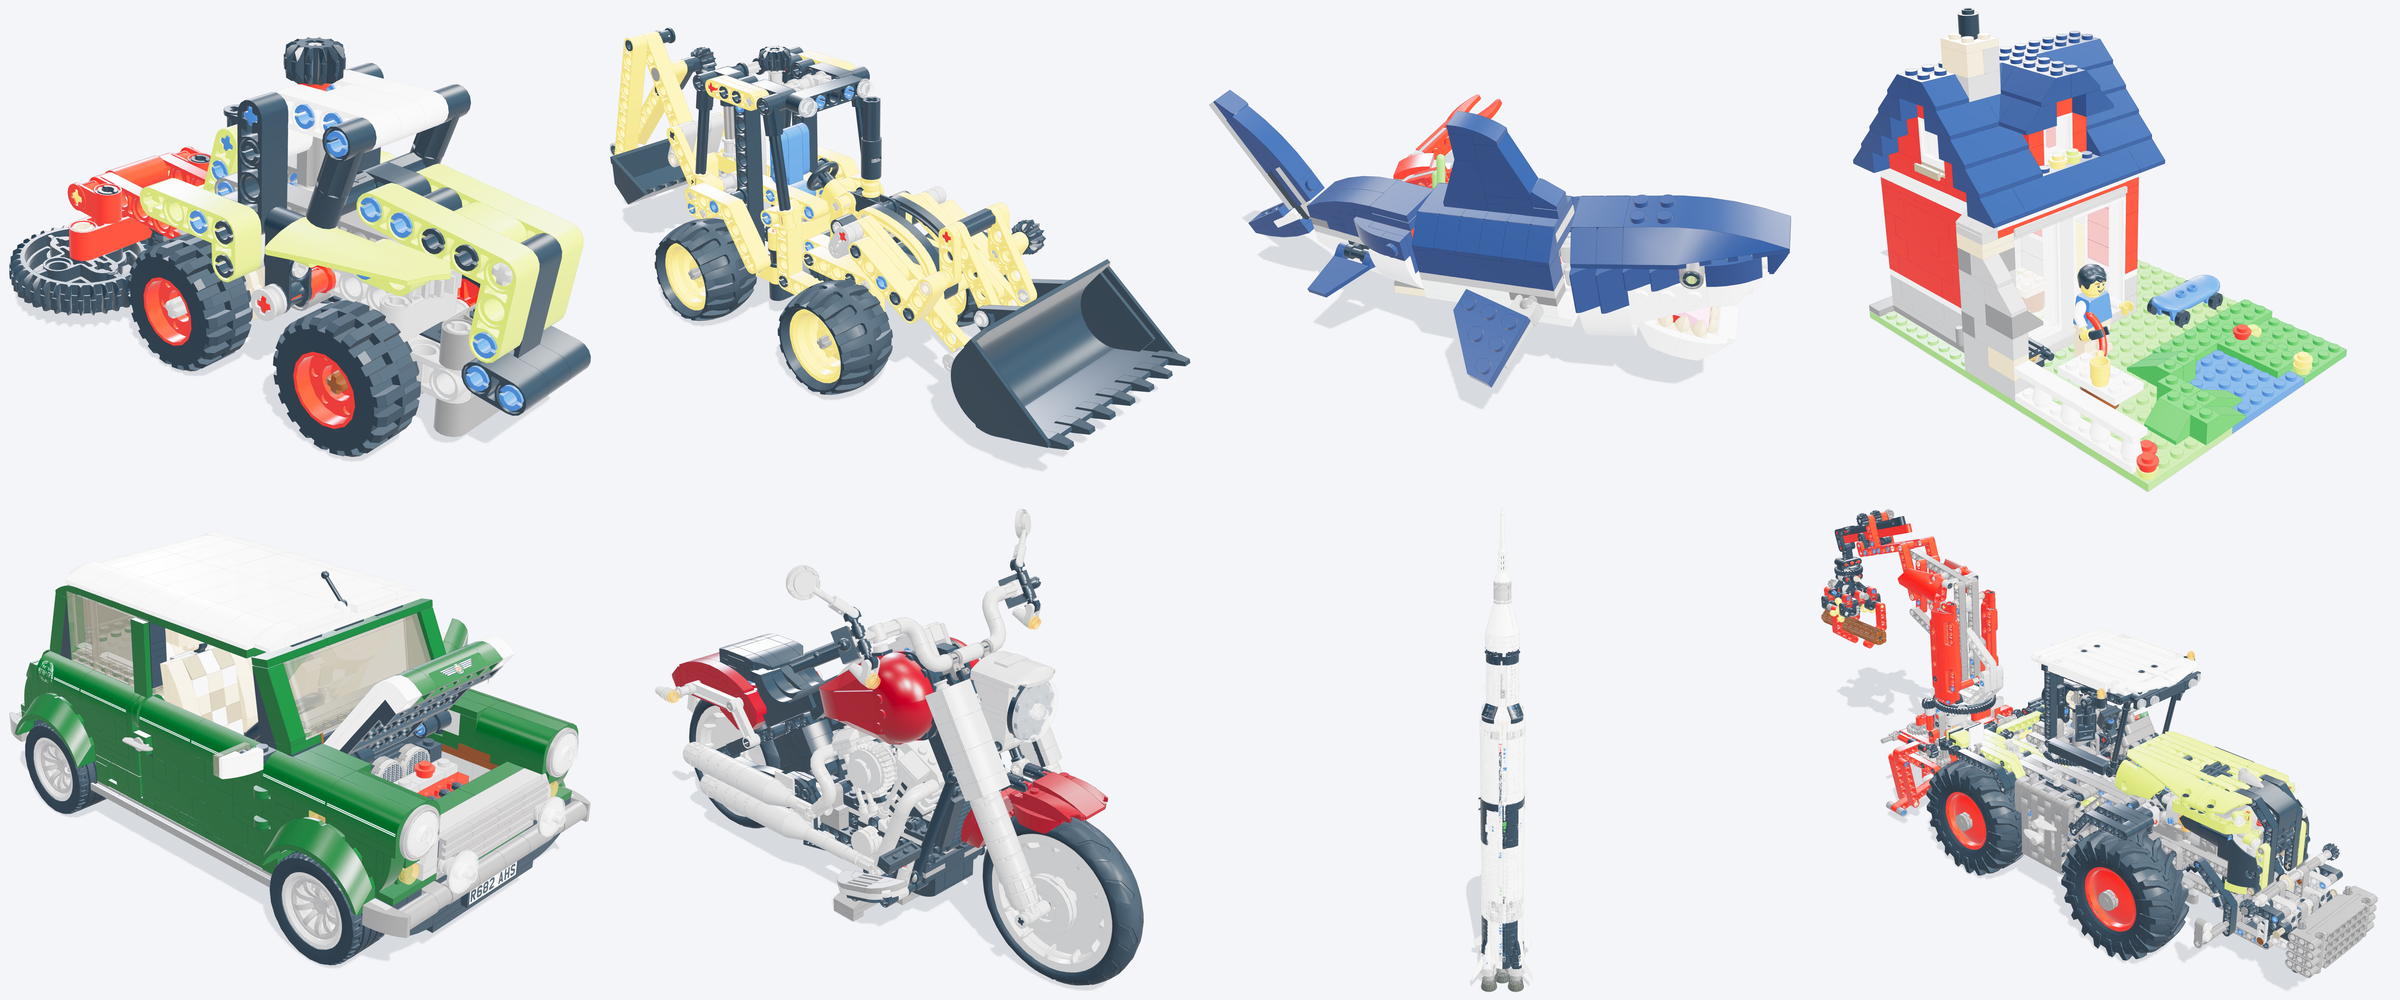
\includegraphics[width=.92\textwidth]{figures-v2/sources.png}
\plateid{fig:sources}
\end{figure*}

\section{Introduction}
An assembly question is meaningful only if both the referenced part and
the permitted evidence are explicit. A color judgment from a rendering,
a lookup in a connector record, and a count of graph components may
refer to the same brick while measuring different operations. A correct
graph answer also does not establish a feasible extraction or stability
under gravity. Combining such scores without their observation
contracts can obscure what a model actually demonstrated.

BrickAtlas uses unchanged original source assemblies
(Fig.~\ref{fig:sources}) and source-local numbers such as
\texttt{B0001} to align views, records, graphs and display edits.
This supports inspectable comparisons about an exact instance. It
does not, by itself, prove that failures can be localized to independent
cognitive modules. Such a claim would require targeted interventions,
non-target stability and evidence restoration.

LDraw-2 also addresses a concrete measurement problem in the preceding
frozen question generator. In graph deletion and author-step lookup,
the correct numerical choice was always second-smallest. Ordered
reference arrays additionally encoded answers for type correspondence
and neighbors when those arrays were available in the input. Together,
these four rules predict 268 of 617 frozen public items. This establishes
availability of shortcuts, not that a learned model used them.
The old release and any historical evidence remain unchanged.

Our contributions are threefold. First, we preserve an attributable
corpus with instance-aligned observation contracts and a complete
question-level audit. Second, we repair demonstrated shortcuts and
provide a single whitelist boundary with actual request snapshots and
independent oracles. Third, we release controlled evidence comparisons,
paired rendering and a review workflow that makes remaining ambiguity
explicit. The present development manuscript reports measured corpus
and software properties; its model and human result cells remain blank.

\section{Related Work}
\paragraph{Brick assembly and spatial reasoning.}
BrickNet~\cite{kulits2026bricknet} learns graph-backed generative brick
assembly. We reuse its public connector implementation for auditing
fixed source placements. Our immediate research question concerns
answers and editing contracts on those placements, so our checks do
not replicate its generative evaluation.
LEGO-Puzzles~\cite{tang2025legopuzzles} studies elementary spatial
questions and multi-step planning. Its public abstract motivates a
related capability question; our narrower contribution is the explicit
separation of rendered, source, graph and edit evidence. We do not infer
absence of instance identity or diagnostic support in neighboring work.

\paragraph{Physical evaluation.}
PhyBlock~\cite{ma2025phyblock} evaluates physical understanding and
planning in robotic block assembly. LDraw-2 currently specifies local
graph operations and visibility transitions at fixed poses.
Consequently, physical success under PhyBlock's contract and exact
success here are different measured outcomes. Detailed capability
comparisons require full protocol alignment and remain to verify.

\paragraph{Diagnostic benchmarks versus capability benchmarks.}
CLEVR~\cite{johnson2017clevr} and GQA~\cite{hudson2019gqa} make
compositional question operations explicit. This motivates documenting
our operations, but neither their balancing nor their diagnostic
validity transfers automatically. A capability score describes
performance under an observation contract. Diagnostic localization
requires additional evidence that a controlled change affects the
intended component while other components remain stable.
LDraw-2 supplies intervention infrastructure; this validity study has
not been run. Table~\ref{tab:related} separates research questions from
verified evidence instead of assigning unsupported negative
capabilities to other benchmarks.

\begin{table*}[t]
\centering\small
\caption{Conservative positioning. External rows describe verified
high-level topics. ``To verify'' means no full capability comparison
has been established; it does not mean an absent capability.}
\label{tab:related}
\begin{tabularx}{\linewidth}{lXXX}
\toprule
Work & Research question & Observation / evaluation contract & Evidence in this study\\\midrule
BrickNet & Generative brick assembly & Connectivity-based build programs & Public connector implementation reused; finer comparison to verify\\
LEGO-Puzzles & Multi-step spatial reasoning & Visual questions and assembly planning & Public abstract checked; detailed identity/diagnosis support to verify\\
PhyBlock & Physical understanding and planning & Robotic 3D block assembly & Public abstract checked; fine-grained protocol comparison to verify\\
CLEVR / GQA & Compositional visual question answering & Images and explicit question operations & Motivation only; no transferred diagnostic validation\\
LDraw-2 & Separate instance-aligned competencies & V / S / G / E, one contract per item & Full software audit; model, human and diagnostic studies unrun\\
\bottomrule
\end{tabularx}
\end{table*}

\section{Representation and Task Contracts}\label{sec:contracts}
\subsection{Source Identity and Observation Permissions}
An expanded assembly contains instances $(b_i,p_i,c_i,T_i,h_i)$:
identity, source part type, color, transform and hierarchy path.
A complete reference is the source SHA256 and instance identity;
the display label \texttt{B0001} is unique only within that source.
Nested MPD transforms and dependency geometry are retained under the
LDraw specification~\cite{ldraw}. Independent reparsing verifies type,
color, transform and hierarchy for all \VTwoParts{} instances.
The interactive viewer uses Three.js~\cite{threejs}.

V items receive numbered PNG bytes and question/options, with no
source attributes. S items receive required coordinates, coverage
flags, evidence scope or author-step rows. G items receive a connector
record or local edges. E items receive action facts and budget.
None receives reference answers. The human review website additionally
exposes internal evidence and is therefore not a model test sandbox.

The recognized connector graph is the undirected projection of
matched part pairs. Repeated connector records are deduplicated for
graph operations. Missing connector definitions remain unknown
evidence, and a scene may contain legitimate separate objects.
Intersection candidates without a recognized mating pair are retained
for inspection; they are neither confirmed defects nor force estimates.

\begin{table*}[t]
\centering\footnotesize
\caption{All eleven families and their direct measurement contracts.
A/M/P/GI denote atomic, metacognitive, procedural and graph-internal
organization; they are not calibrated difficulty levels.
$\dagger$: constant semantic response/program;
$\ddagger$: explicit evidence reading or arithmetic.}
\label{tab:operators}
\begin{tabularx}{\linewidth}{lrrlXXXX}
\toprule
Family & $N$ & Layer & Input & Measurement & Direct operation & Necessary input & Shortcut control\\\midrule
Color & 73 & A & V & Perception & Identify color & Numbered image & Request whitelist\\
Part type & 67 & A & V & Perception & Match source type & Numbered image & No reference order\\
Distance$^\ddagger$ & 73 & A & S & Evidence reading / arithmetic & Euclidean minimum & Centers (mm) & No source path\\
Interface$^\ddagger$ & 87 & M & G & Evidence reading & Read family & Connector record & Fixed five options\\
Neighbors & 73 & M & G & Graph operation & One-hop exact set & Local edges & No reference order\\
Graph deletion & 73 & GI & G & Graph operation & Delete; count components & Nodes and local edges & Integer output\\
Coverage$^\ddagger$ & 17 & M & S & Evidence reading & Read support flag & Coverage rows & Minimal row fields\\
Evidence limit$^\dagger$ & 24 & M & S & Evidence scope control & Fixed scope response & Available evidence & Report fixed prior\\
Step lookup$^\ddagger$ & 55 & P & S & Evidence reading / lookup & First index lookup & Author-step rows & Legal balanced ranks\\
Step sequence$^\dagger$ & 17 & P & E & Execution contract & Follow fixed program & Facts and actions & Report fixed prior\\
Restoration & 58 & P & E & Execution contract & Restore visibility & Facts and actions & Remove redundancy\\
\bottomrule
\end{tabularx}

\end{table*}

\subsection{Eleven Separate Families}
Table~\ref{tab:operators} states each required input and operation.
Color and part-type correspondence are the only two visual families.
Their oracle uses source color or part-type equality, which does not
certify that a human can distinguish the rendered alternatives.
Distance uses supplied bounding-box centers in millimeters and
Euclidean arithmetic. Candidates are deterministically hash-sampled;
the task does not estimate distances from pixels.

Interface directly reads \texttt{connectorRecord.family}; coverage
reads a false support flag; author-step lookup finds the first supplied
expanded index containing the target. These are evidence controls.
Neighbors extracts the exact one-hop candidate set. Graph deletion
removes a named vertex from the supplied local graph and counts
remaining components, including isolated nodes. It is graph-internal,
not a cross-modal task or physical extraction test.
The local deletion graphs contain only 5--9 nodes and 2--6 unique
edges; their source assemblies can be much larger.

Evidence-limit items all answer ``Not established by this evidence''
to a gravitational-stability claim. All seventeen source-sequence
items also share the same six-step response program. Their scores
must be reported as fixed-answer or fixed-program controls.
Restoration instead follows the public missing/present facts to
restore one numbered instance's visibility.

The four organization layers contain 213 atomic, 201 metacognitive,
130 procedural and 73 graph-internal items. Response formats are
396 single-choice, 73 multiple-choice, 73 integer and 75 action items.
These counts reflect applicability, not balanced quotas.

\subsection{Executable Scene Edits}
For facts $F$, an action requires $R_a\subseteq F$, forbids
$B_a\cap F\ne\varnothing$, and costs $c_a$ within the remaining
budget. Accepted execution applies
\begin{equation}
F'=(F\setminus D_a)\cup A_a .
\end{equation}
The display changes visibility at original source poses. Unknown
actions, violated prerequisites, forbidden facts and over-budget
execution are rejected without applying that transition.
Success requires all goal facts and no prohibited facts.

Figure~\ref{fig:replay} shows the same six author-window states as the
preserved source replay for set 42102. The v2 facts and semantic
program remain unchanged. This is following a supplied author order,
not discovering a collision-free insertion sequence. The supplement
also shows accepted and rejected restoration at the original poses.

\begin{figure}[t]
\centering

\includegraphics[width=.32\linewidth]{figures-v2/sequence-1.jpg}
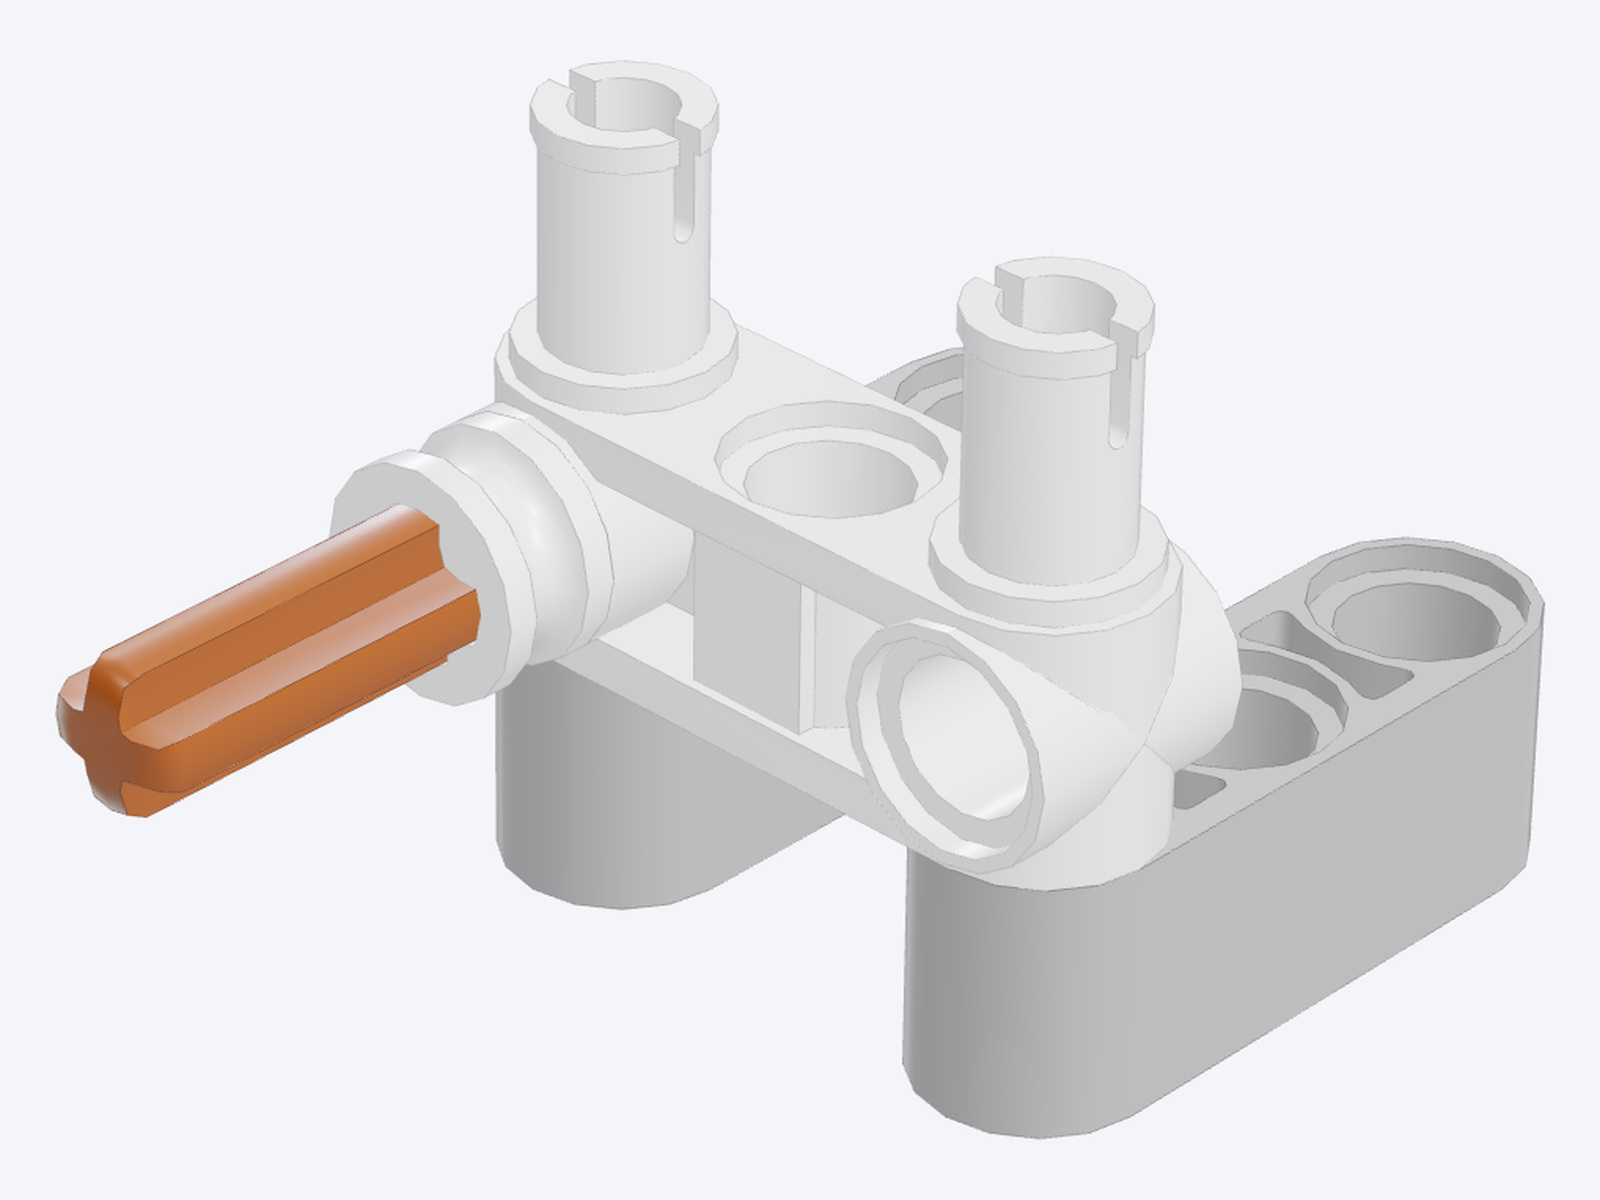
\includegraphics[width=.32\linewidth]{figures-v2/sequence-2.jpg}

\includegraphics[width=.32\linewidth]{figures-v2/sequence-3.jpg}\\
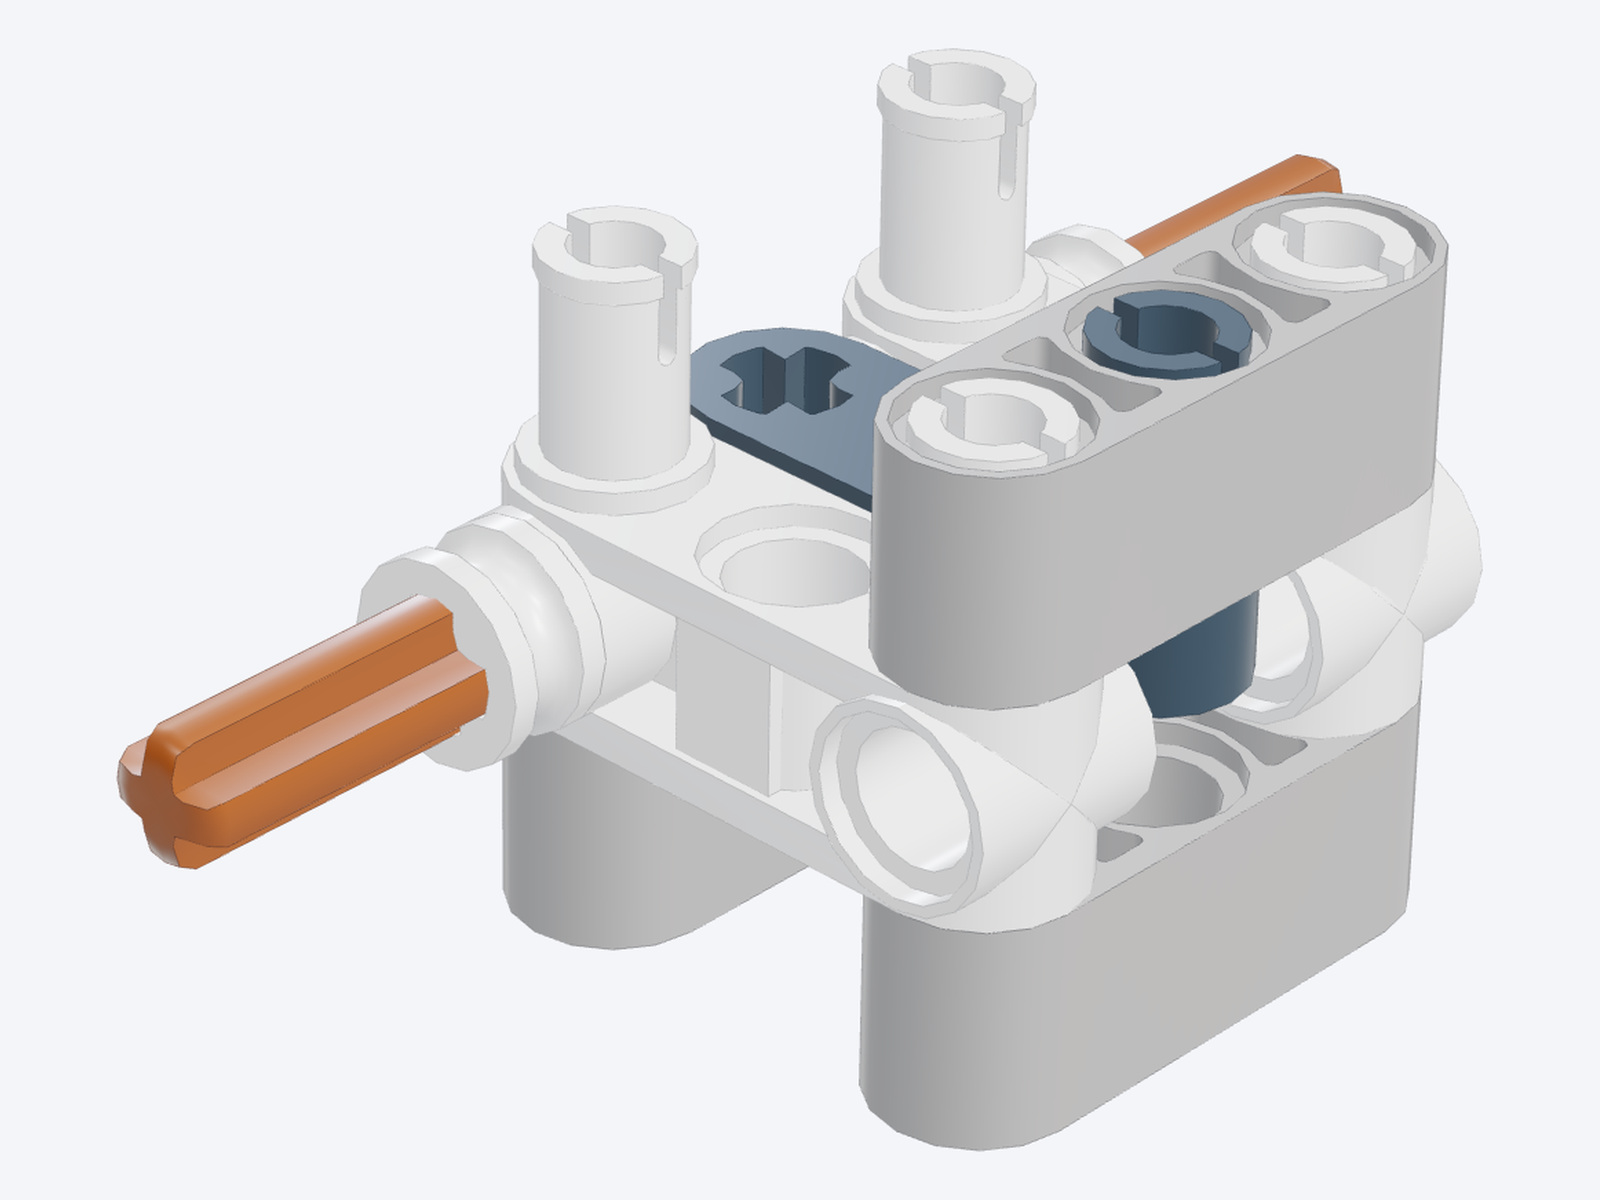
\includegraphics[width=.32\linewidth]{figures-v2/sequence-4.jpg}
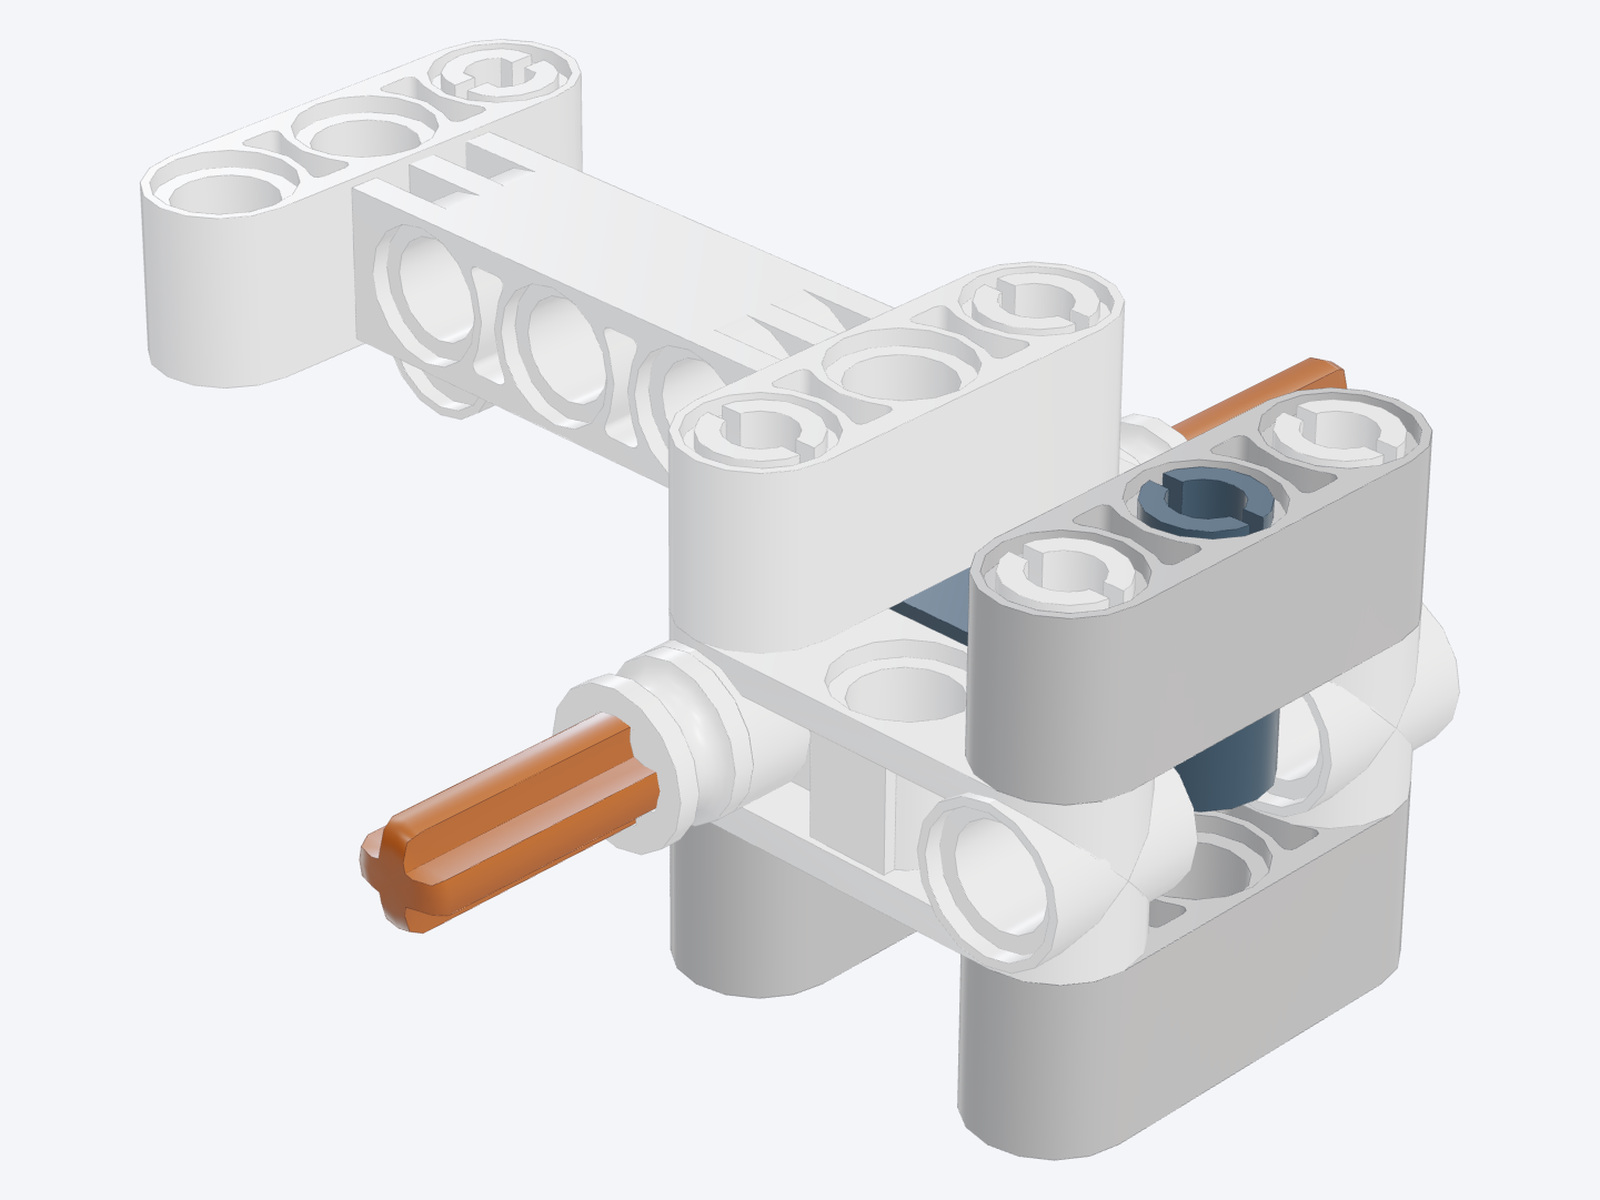
\includegraphics[width=.32\linewidth]{figures-v2/sequence-5.jpg}

\includegraphics[width=.32\linewidth]{figures-v2/sequence-6.jpg}
\plateid{fig:replay}
\end{figure}

\section{Measurement Repair and Corpus Analysis}
\subsection{Shortcuts and Request Isolation}
For author-step lookup, four distinct legal indices now give correct
semantic ranks 14/14/14/13. Graph deletion has a boundary constraint:
63 of 73 answers equal the maximum legal component count. Four
distinct legal numeric choices would make these answers largest,
replacing one shortcut with another. We therefore use exact integer
responses for all 73 items, preserving graphs and semantic answers.
This is an explicit output-format change, so old numerical-choice
scores cannot be silently compared as equivalent conditions.

Type-match internal references are globally hash-permuted; correct
reference positions are 14/13/13/13/14. References for all families are
excluded from actual model requests, eliminating the reference-slice
channel. Internal accidental matches remain reported in the audit.
Interface now always offers all five connector families; the old
answer-dependent option count otherwise exposed stud answers.

The unique serializer admits only a fixed system prompt, English
question, format, necessary input, anonymous option IDs/labels and
declared image bytes. It removes internal references, target and
capability metadata, answer fields, source paths, option values and
redundant missing-instance lists. Public preconditions remain because
they define the E contract. The runner rejects internal bundle paths,
including realpath aliases. Every actual wire request is saved and
hashed before an optional API call.

\subsection{Source Scale and Task Dependence}
The retained corpus has 24 distinct set families and 15,334 instances.
Source sizes range from 53 to 1,978, with median 274.
D1 is at most 150 instances; D2 is 151--400; D3 is 401--1,000;
D4 exceeds 1,000. Table~\ref{tab:bands} reports the measured cross-tab.
Only two sources are in D3. Larger sources generate more items
(Pearson $r=0.9498$, Spearman $\rho=0.9049$), partly by construction.
Neither association measures cognitive difficulty.

\begin{table}[t]
\centering\small
\caption{Measured size-band by observation counts. Source size and
single-item difficulty are separate quantities.}
\label{tab:bands}\begin{tabularx}{\linewidth}{Xrrrrrr}
\toprule
Band & Sources & V & S & G & E & Total\\\midrule
D1 & 5 & 17 & 21 & 33 & 12 & 83\\
D2 & 9 & 34 & 47 & 69 & 25 & 175\\
D3 & 2 & 14 & 15 & 23 & 7 & 59\\
D4 & 8 & 75 & 86 & 108 & 31 & 300\\
\bottomrule
\end{tabularx}

\end{table}

Among 593 items with nonempty operands, 148 share their exact
source-local operand set with another item. The focal color/type/
distance/restoration families contain 271 items over 73 source-local
targets. Shared instances motivate paired reporting and source-cluster
uncertainty; repeated labels across sources are not identical objects.
No training split or pretraining-contamination estimate is established.

\subsection{Semantic Answer Concentration}
Figure~\ref{fig:priors} shows every family's in-corpus majority share.
Instance-valued responses use source-qualified identities (orange);
their low shares are not comparable to a reusable global semantic
class and do not establish diversity of reasoning.
The graph-deletion majority is 4 on 44/73 items (60.27\%).
Evidence limit and the six-step program have 100\% semantic priors.
Across the 396 single-choice items, always A scores
\VTwoAlwaysA\% and uniform sampling has expected accuracy
\VTwoUniform\%. These descriptive controls are not held-out results.

\begin{figure}[t]
\centering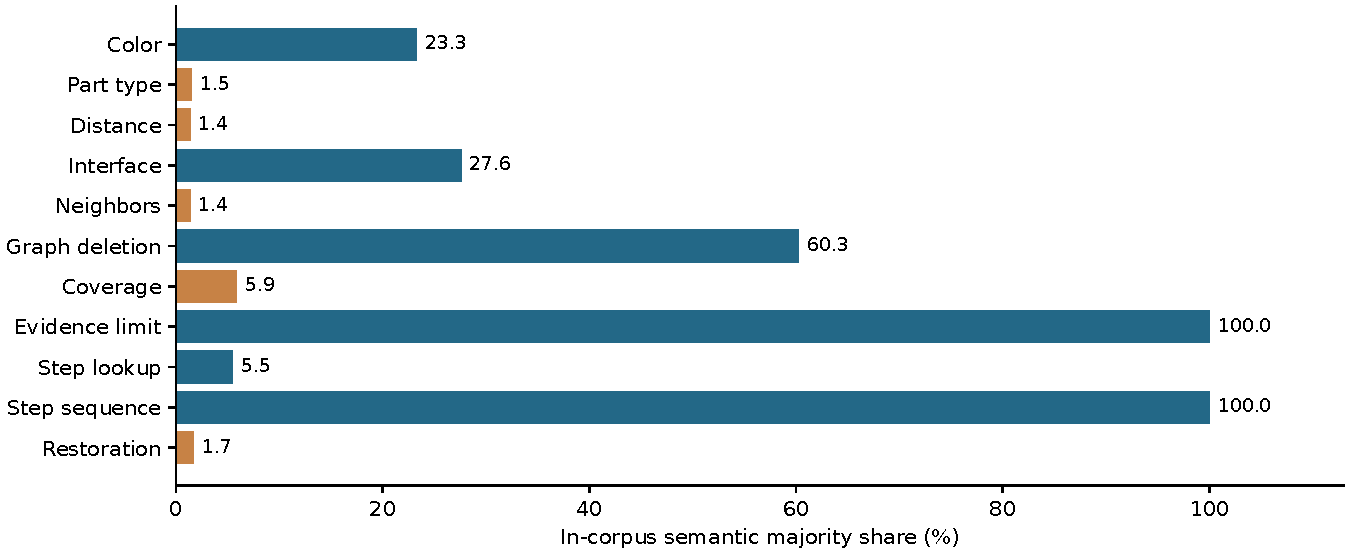
\includegraphics[width=\linewidth]{figures-v2/answer-concentration.pdf}
\plateid{fig:priors}
\end{figure}

\section{Evaluation Protocol and Evidence Status}
\subsection{Controlled Observations}
Standard inputs cover V=140, S=169, G=233 and E=75.
Contrary to the prior planning text, the frozen standard visual images
already isolate operands. V2 adds full-scene and background-mask images
with identical camera, scale, lighting and label projection; the crop
separately refits the camera. Figure~\ref{fig:pairs} shows these three
observations, left to right, for one type-match item. A crop changes
both visibility and scale, so it is not a pure background-effect estimate.

\begin{figure*}[t]
\centering
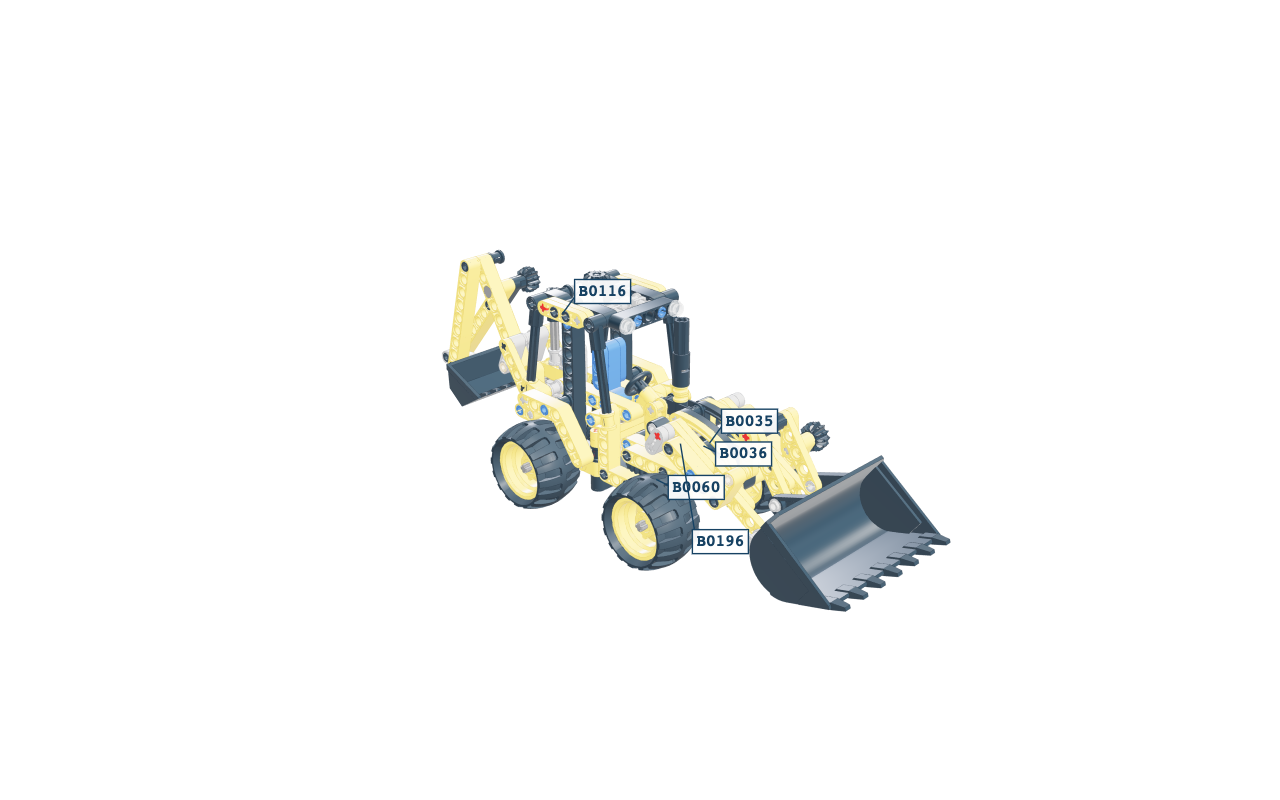
\includegraphics[width=.32\textwidth]{figures-v2/paired-full.png}
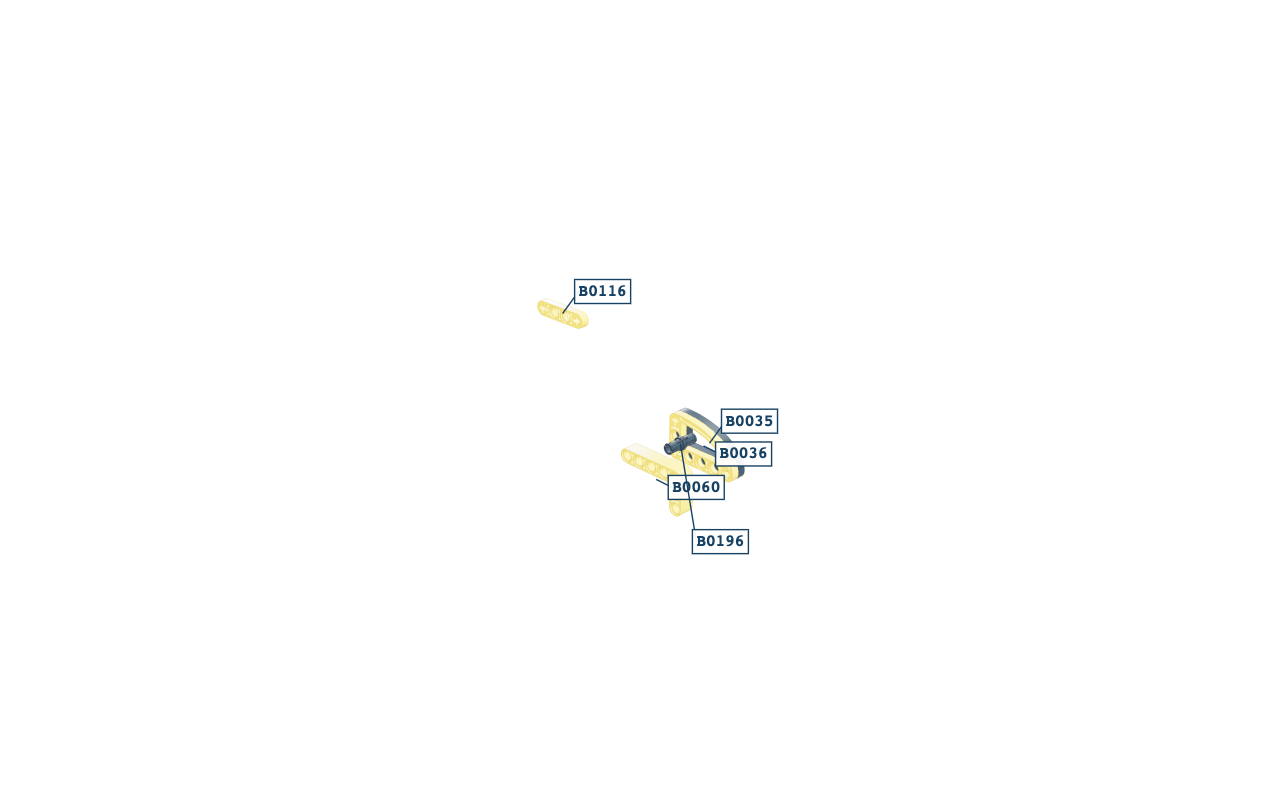
\includegraphics[width=.32\textwidth]{figures-v2/paired-mask.png}
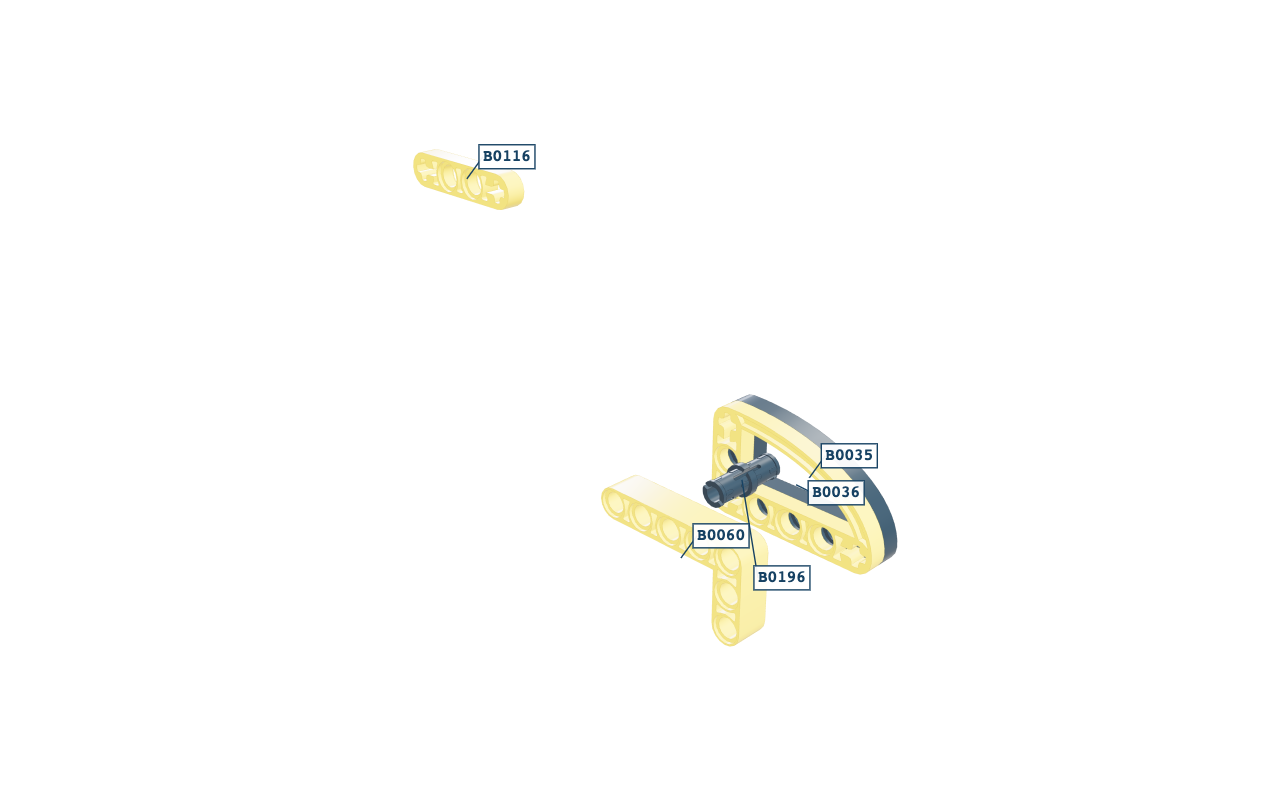
\includegraphics[width=.32\textwidth]{figures-v2/paired-crop.png}
\plateid{fig:pairs}
\end{figure*}

\begin{table}[t]
\centering\small
\caption{Executable conditions and eligible counts. Every blank exact
success cell means not run. Counts are not performance measurements.}
\label{tab:conditions}\begin{tabularx}{\linewidth}{Xrr}
\toprule
Condition & $N$ & Exact success\\\midrule
standard & 617 & \\
text-without-image & 140 & \\
graph-edges-withheld & 146 & \\
full-scene & 140 & \\
background-mask & 140 & \\
operand-only & 140 & \\
choice-order & 469 & \\
edge-order & 146 & \\
id-permutation & 576 & \\
wrong-image & 140 & \\
camera-perturbation & 140 & \\
color-nuisance & 67 & \\
multi-view & 140 & \\
graph-intervention & 146 & \\
\bottomrule
\end{tabularx}

\end{table}

The 14 conditions in Table~\ref{tab:conditions} cover 3,147 eligible
item-condition pairs. Edge withholding and ordering apply to 146
edge-based items, excluding 87 interface records. Graph interventions
remove a neighbor pair or join surviving components; independent
recomputation confirms a changed answer for every eligible item.
These are hypothetical evidence graphs, not repaired CAD sources.
ID permutation applies to 576 labeled items; the remaining 41
controls contain no B-number. Choice ordering applies to 469 items.
Fixed two-view access is executable; an adaptive camera/tool agent is
not implemented by that condition.

\subsection{Scoring, Adapters and Statistical Interpretation}
Single choice requires exact \texttt{choiceId}; multiple choice
requires the exact set without duplicates. Graph deletion requires
an exact safe JSON integer in \texttt{value}. E requires legal complete
execution reaching all goals. Format validity and goal success are
reported separately and do not demonstrate mechanical planning.
Missing, malformed, refused and timed-out responses remain failures.

Six candidate adapter configurations specify exact model IDs,
transport, decoding, prompts, image size, timeout and revision gates.
Moving aliases require an actual frozen revision before live use.
Both OpenAI-compatible and Anthropic wire formats are implemented.
Images are deterministically letterboxed to 1280 by 800 pixels.
Each run saves code/config hashes, git revision, actual requests,
responses, usage, latency and strict scores. There is one attempt
per item, no hidden retry and no automatic JSON repair. Unknown
prices or token usage remain null.

\begin{table}[t]
\centering\small
\caption{Prospective candidate-family exact success (\%).
All model result cells are blank. The supplement gives adapter IDs
and additional family, resource and review tables.}
\label{tab:models}\input{tables-v2/plan-models.tex}
\end{table}

Micro accuracy averages item successes; source macro first averages
eligible items within each source and then averages eligible sources.
The primary paired estimand is the per-family A-minus-B source-macro
difference; micro is secondary. The protocol specifies 10,000 paired
source-cluster bootstrap resamples, seed 20260918 and percentile 95\%
intervals. Correct-to-wrong and wrong-to-correct transitions must also
be reported. Repeated items or views are not independent clusters.

Compare correct, absent and mismatched images; compare full, masked,
cropped and text-only evidence. An interval containing zero permits
only ``no stable gain detected.'' It does not establish equivalence,
zero contribution or absence of all scale effects. No equivalence
margin has been preregistered. Edge withholding tests information
dependence; answer-changing interventions together with invariance
under edge ordering provide stronger evidence. These comparisons
must be evaluated by family before any declared aggregate.

Historical replay requires authentic saved v1 wire requests and
receipt provenance. None is presently available for an eligible
comparison. We do not reconstruct an intentionally leaky input and
present it as a historical run.

\subsection{Measured Software Checks and Pending Review}
Independent oracles pass for all 617 items, the public-precondition
solver succeeds on 75/75 E items, and 5,154 negative controls pass.
Path isolation rejects all 24 internal bundles; 617 canaries and
request snapshots pass. All 907 new visual-condition images reproduce
byte for byte across a second capture of all 140 visual items.
There are 617 actual standard wire snapshots and 14 condition
canaries, produced without model API calls.

These checks establish software consistency and observation
reproducibility. The required human queue contains every visual item
plus 111 other flagged tasks, with reviewer, decision and rationale
still empty. A separate queue binds all 573 physical candidates to
source hashes and exact part pairs. Human feedback can be exported,
reviewed and reimported with version/content validation. Automated
checks never create human approvals.

\section{Discussion and Limitations}
No family currently requires chaining two observation contracts.
Instance alignment supports modular comparisons, but diagnostic
localization remains unvalidated until targeted failures, non-target
stability and evidence restoration are tested. Products or regressions
of isolated module scores cannot establish unmeasured integration.

The corpus is small, uneven and potentially familiar from pretraining.
Large assemblies do not automatically make operand-isolated items
hard. Several families are elementary evidence controls, and the
fixed six-step program has no response diversity. Repaired shortcuts
do not prove universal absence of non-target cues. Near-identical
part variants, lighting-dependent colors and occlusion still require
all-item visual adjudication.

OMR provenance is not physical certification. Unsupported definitions,
connector tolerances, approximate intersection geometry and the 573
pending pairs prevent claims of complete physical validity. Display
replay neither simulates force nor proves insertion feasibility.
All original sources and v1 publication assets remain frozen; any
future correction must preserve their attribution and version history.
The present release is reviewable development infrastructure, with
model rankings, human reliability and physical conclusions still open.

\bibliographystyle{ieeenat_fullname}
\bibliography{references-v2}
\end{document}
